% For formatting purposes only 
\setcounter{chapter}{6}
\setcounter{section}{7}
\setcounter{subsection}{2}
%\listofalgorithms - think about it ...
%--------------
%- COPY START -
%--------------

\subsection{(W) Mission Control Run}\label{s:missionControlRun}
    \noindent Cover algorithm outer run in multiple decision frames (As bonus mark decision points for rule engine \emph{decision points}):
    \begin{itemize}


        \item Trajectory selection criteria in inner avoidance run
        \item Complete mission control run, including decision invocation conditions
        \item Basically MissionControl.runMissionOnce() function in detail

    \end{itemize}

    \begin{figure}[H]
	    \centering
        \begin{subfigure}{0.48\textwidth}
	        \centering
            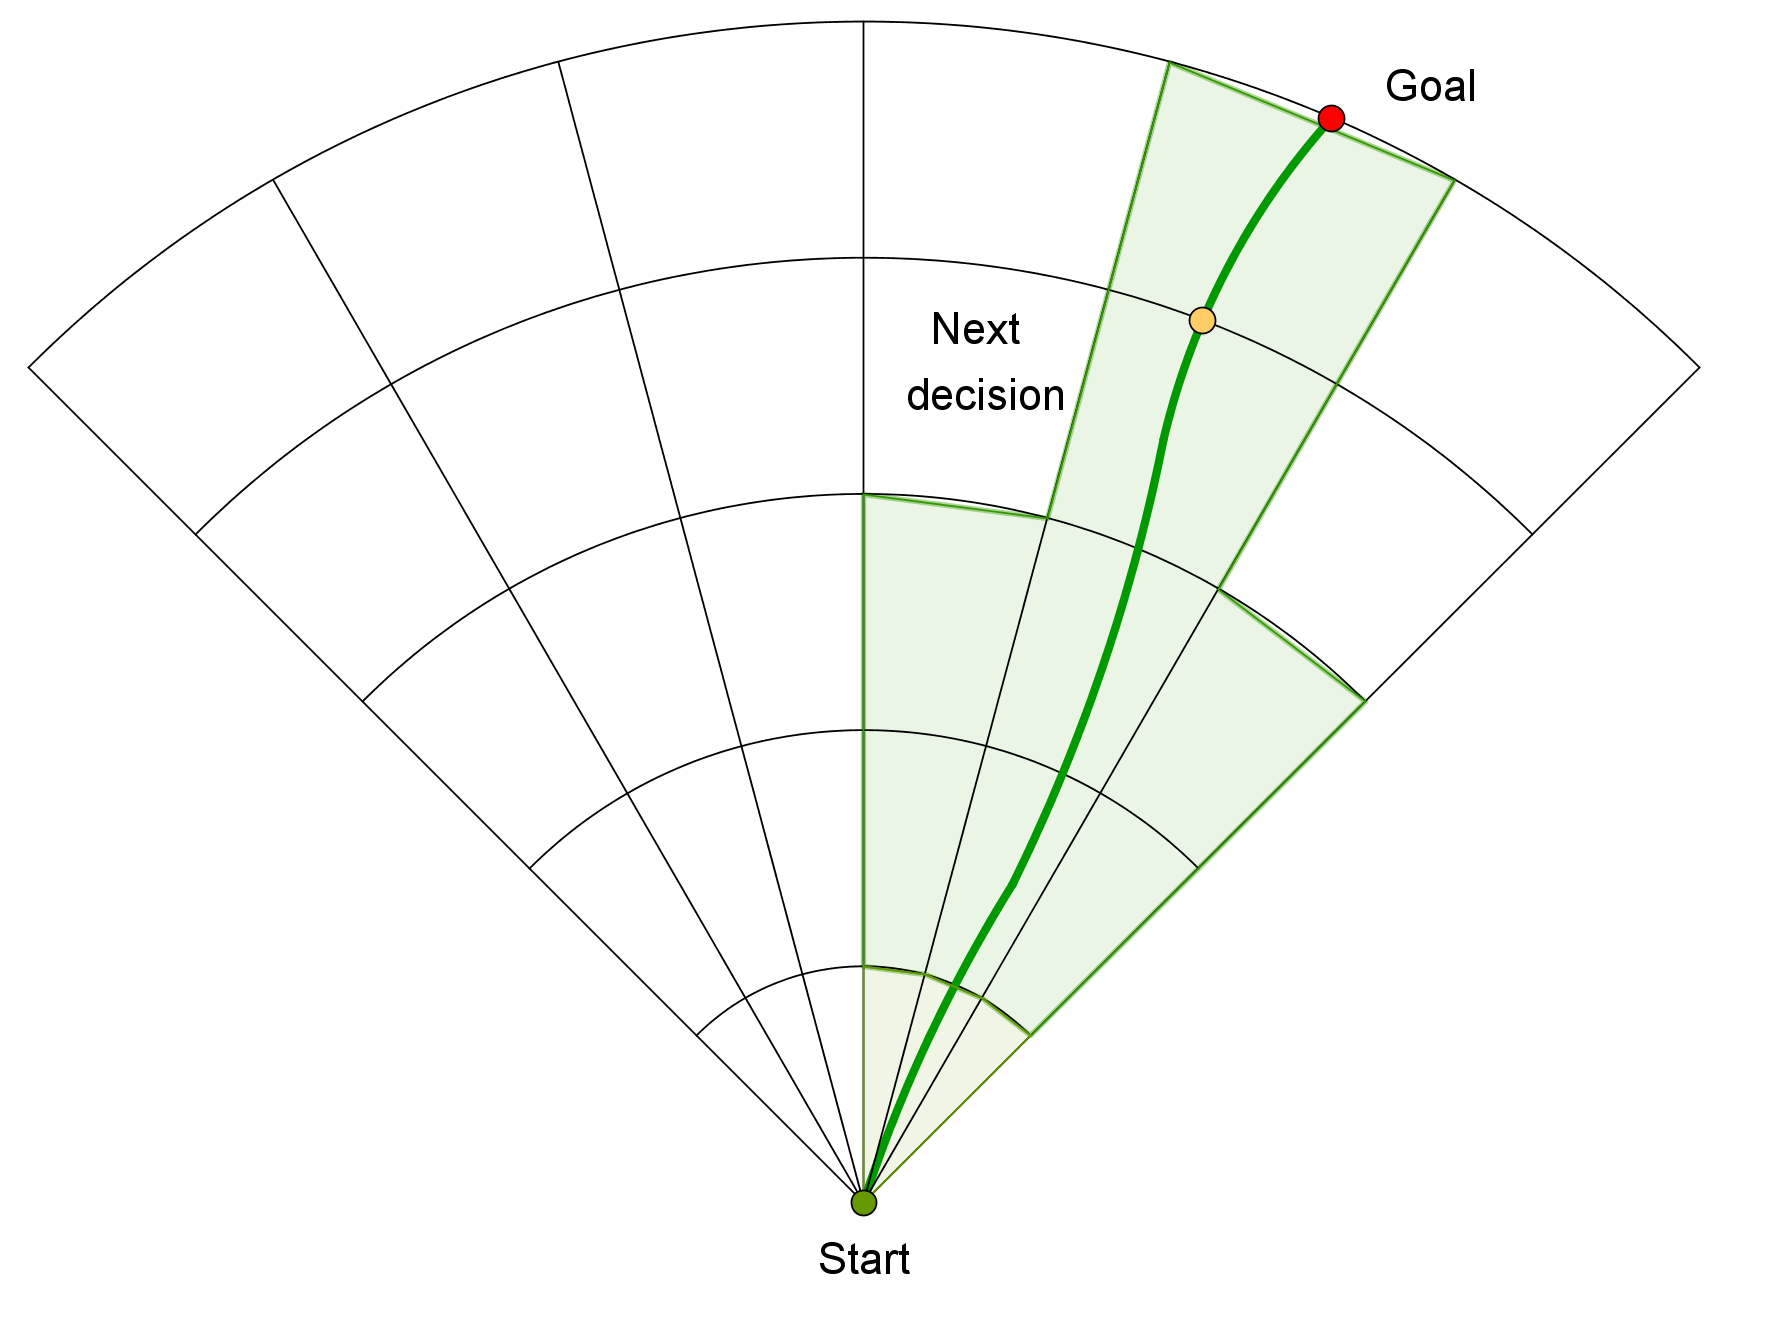
\includegraphics[width=0.9\linewidth]{\FIGDIR/CA005PathCalculation}
            \caption{Mission control run example.}
            \label{fig:missionControlRunExample}
        \end{subfigure}
        \begin{subfigure}{0.48\textwidth}
        	\centering
            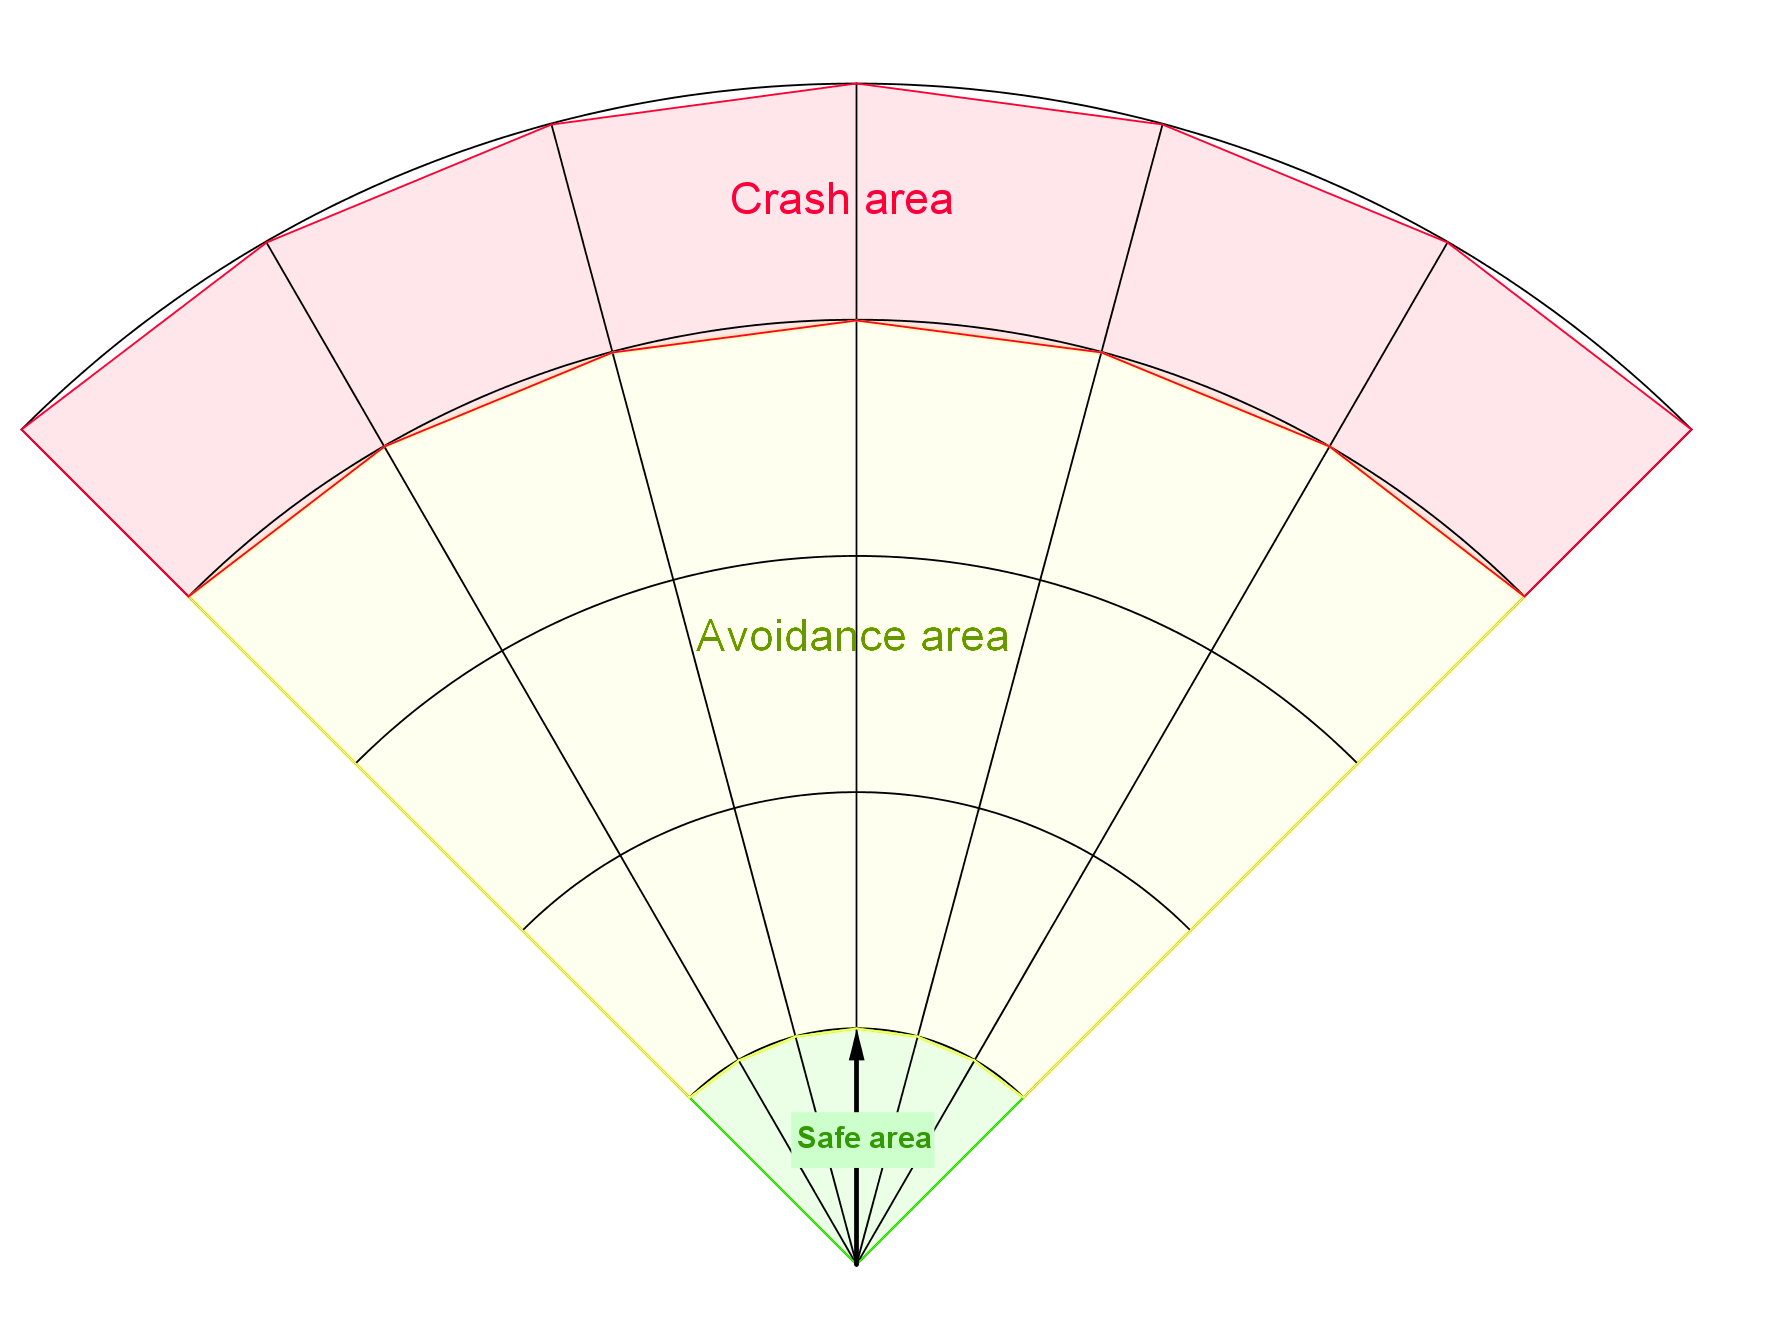
\includegraphics[width=0.9\linewidth]{\FIGDIR/CA006FieldOfViewZones} 
            \caption{Grid zones.}
            \label{fig:gridZonesMissionControl}
        \end{subfigure}
        \caption{Definitions for \emph{Mission Control Run} (outer loop).}
        \label{fig:definitionsForMissionControlRun}
    \end{figure}
    
    


\paragraph{General Concept:}\footnote{Mission Control Run Function Implementation: \url{RuleEngine/MissionControl/MissionControl.m::runOnce(.)}} The \emph{General Concept} is taken from  \cite{sabatini2014navigation,Sabatini2014}, consisting from three main modules:
\begin{enumerate}
    \item \emph{Navigation Loop} - module responsible for \emph{Navigation} providing \emph{Goal Waypoint}.
    
    \item \emph{Data Fusion} (sec. \ref{s:sensorFusion}) - module responsible for \emph{Surveillance Data Feed}.
    
    \item \emph{Situation Assessment} - module responsible for \emph{UAS Safety Evaluation}. 
    
    \item \emph{Avoidance Grid Run} (sec. \ref{s:aviudabceGridRun}) responsible for \emph{Avoidance Path} selection.    
\end{enumerate}

\noindent The main changes to \emph{Navigation architecture} are given in \emph{Mission Control Run} activity diagram (fig. \ref{s:missionControlRun}):
\begin{enumerate}
    \item \emph{Situation Assessment} - added event-based mode switching control. 
   
    \item \emph{Avoidance Run} - added hierarchical evaluation for \emph{Avoidance Path} selection. Prioritizing threat avoidance according to a type. 
\end{enumerate}

\noindent The \emph{Operation Mode} is introduced, based on \emph{Situation assessment} and \emph{Triggering Events} one of following modes are selected in \emph{Avoidance Run}:

\begin{enumerate}
    \item \emph{Navigation Mode} - the \emph{UAS} is navigating trough \emph{Airspace} following \emph{cost effective patterns} and obeying \emph{Airspace Authority} (UTM). The \emph{Navigation Grid} is a instance of \emph{Avoidance Grid} (sec. \ref{s:AvoidanceGrid}) with initialized \emph{Navigation Reach Set} (ex. \emph{Harmonic Reach Set Approximation} (sec. \ref{s:harmonicReachSet})).
    
    \item \emph{Emergency Avoidance Mode} - the \emph{UAS} is \emph{threatened} by obstacle, intruder, hard constraint or \emph{soft constraint}, the \emph{UAS} is navigating trough \emph{Airspace} following \emph{safe avoidance patterns} and \emph{minimizing the impact} of possible damages. The \emph{Avoidance Grid} is term used for \emph{Emergency Avoidance Mode}. The \emph{Avoidance Reach Set Approximation} is initialized in \emph{Avoidance Grid} (ex. \emph{Chaotic Reach Set Approximation} (sec. \ref{s:chaoticReachSet}))
\end{enumerate}

\begin{note}
    Depending on \emph{Operation Mode} the pair of \emph{Avoidance Grid} and \emph{Reach Set} is selected in \emph{Avoidance Run} (sec. \ref{s:aviudabceGridRun}).
    
    
    The \emph{Navigation Grid} and \emph{Avoidance Grid} shares the space segmentation pattern, therefore the \emph{Data Fusion} (sec. \ref{s:sensorFusion}) needs to be evaluated only once. 
\end{note}

\begin{figure}[H]
    \centering
    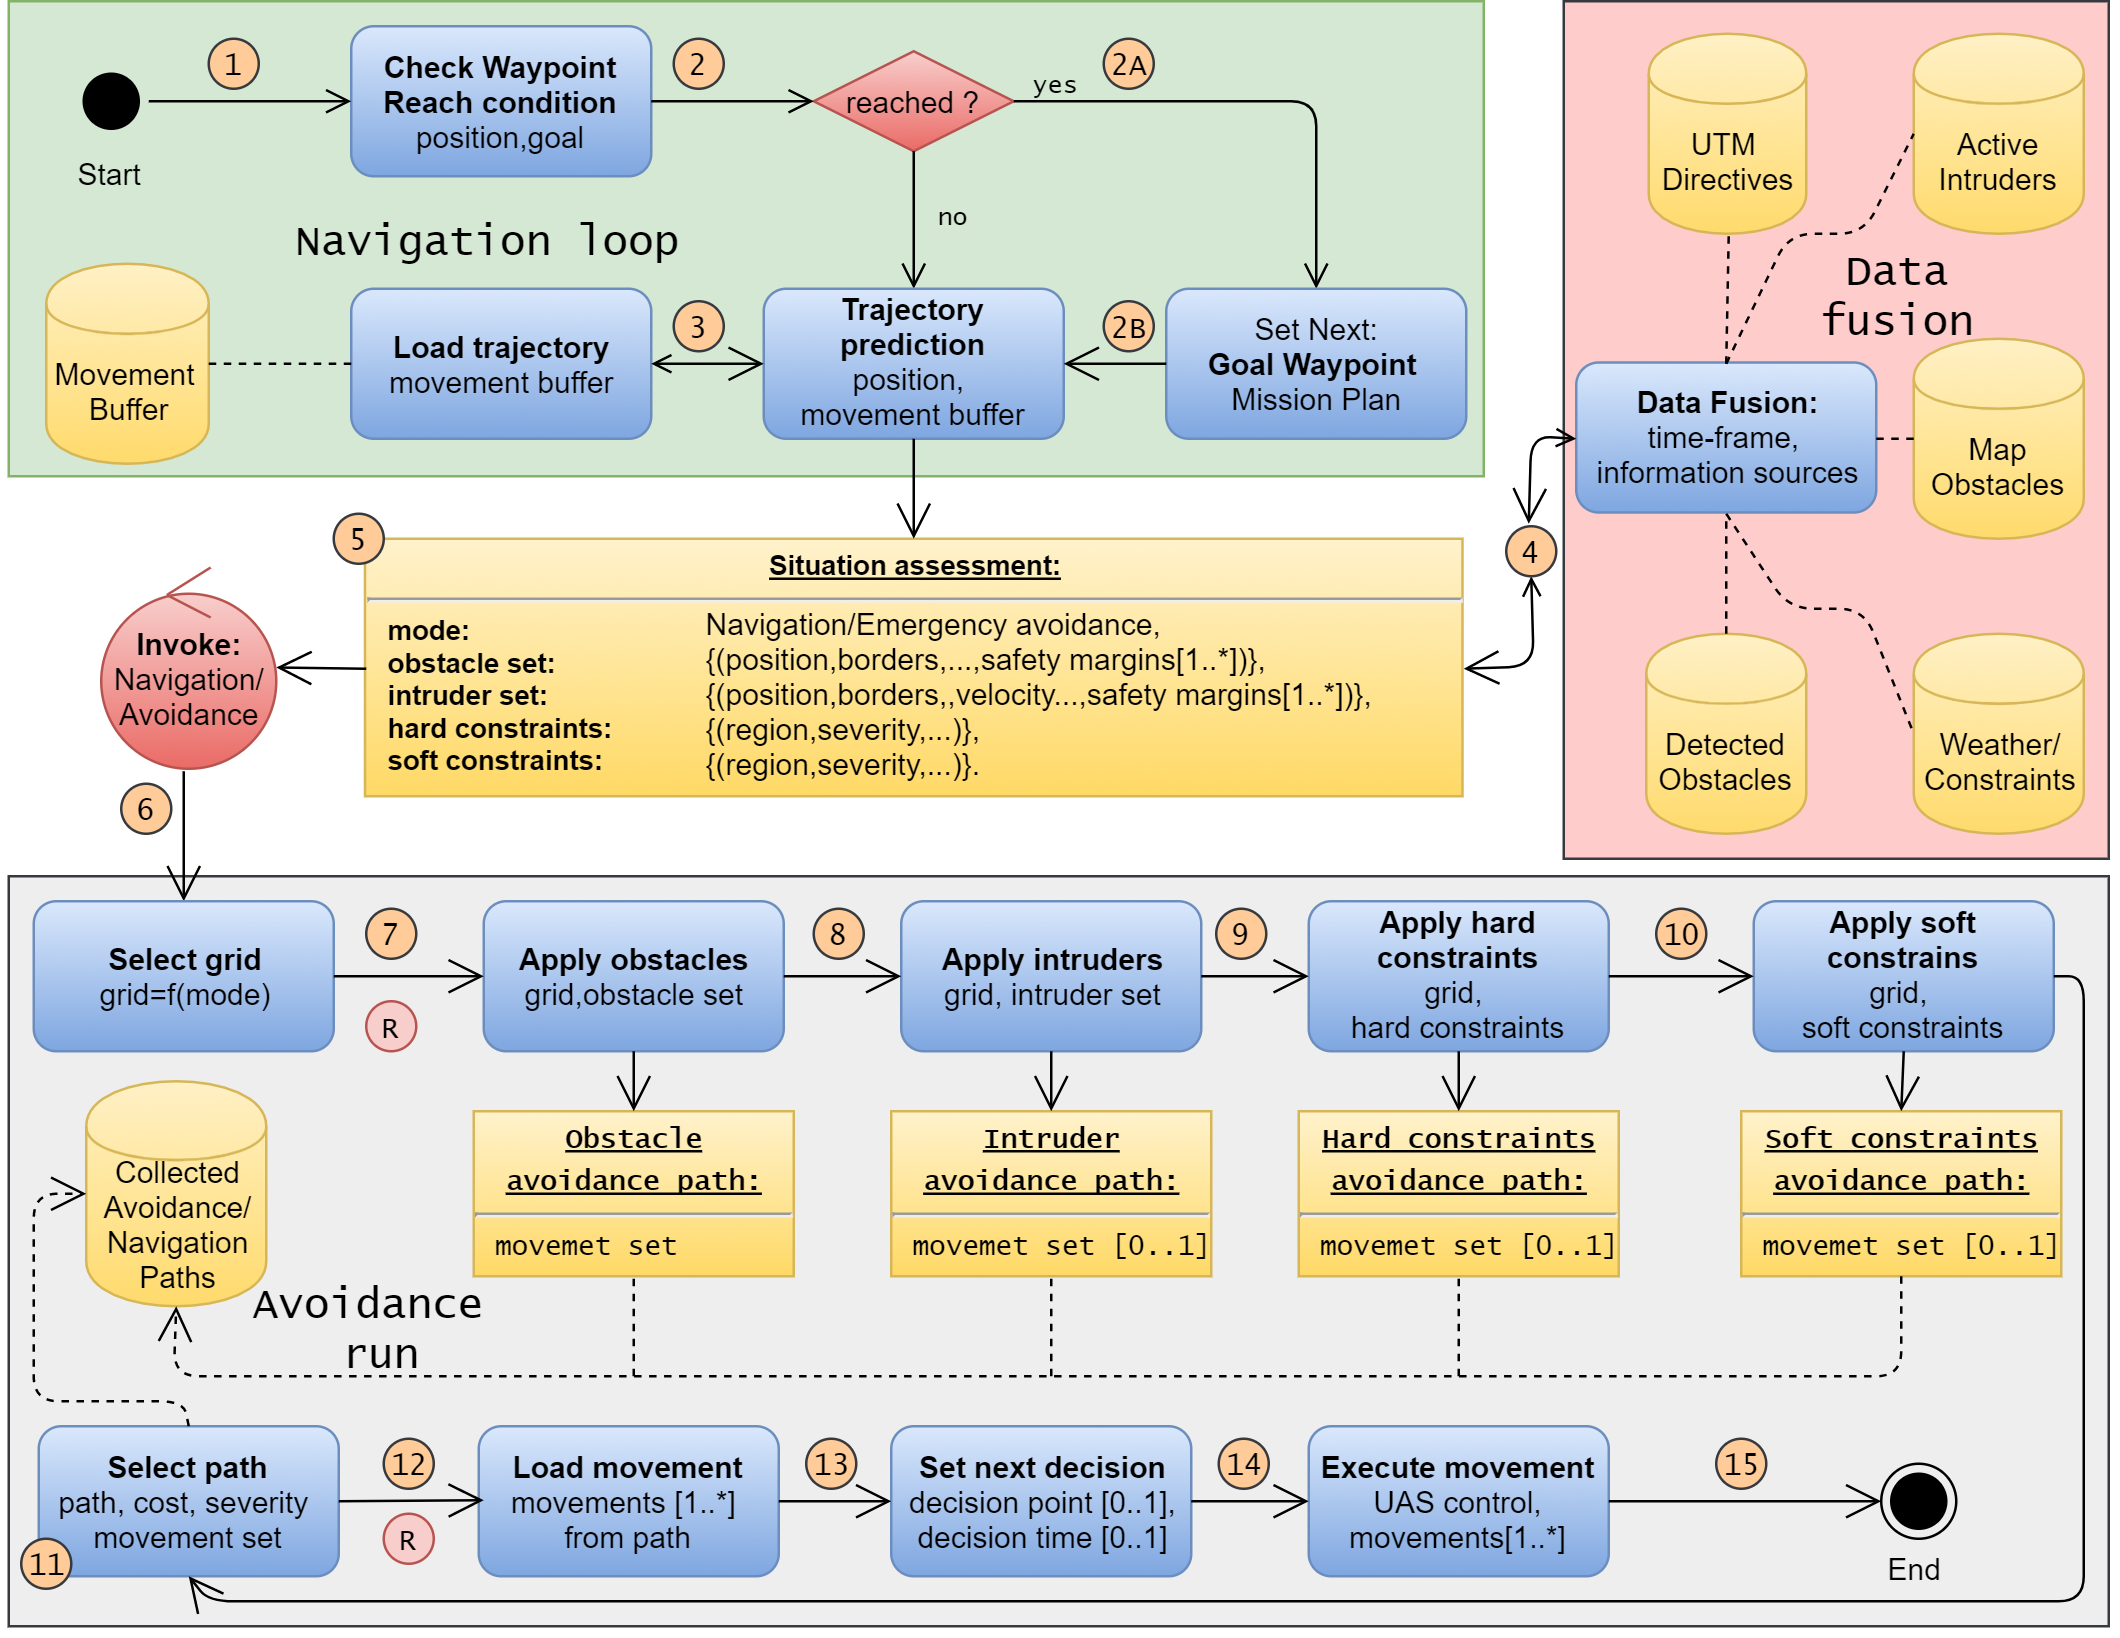
\includegraphics[width=\linewidth]{\FIGDIR/TE026AvoidanceAlgorithmMainLoopRun}
    \caption{Mission control run activity diagram.}
    \label{fig:missionControlRunActivityDiagram}
\end{figure}

\paragraph{Decision Time Frame $[t_i,t_{i+1}[$:} The \emph{Mission Control Run} is executed for \emph{Decision Time Frame} bounded to the \emph{period} of the \emph{UAS executed movement} (fig. \ref{fig:AvoidanceFrameworkConceptNew}).

The \emph{UAS System} (sec. \ref{s:UASNonlinearModel}) controlled by \emph{Movement Automaton Implementation} (sec. \ref{s:movementAutomatonDefinition}) \emph{Planned Movements} can be changed at any time. The real impact on control is shown after the \emph{actual movement} is executed. 

For our \emph{Movement Automaton} movements the average \emph{movement duration} is \emph{1/velocity second} (tab. \ref{tab:movements1}, \ref{tab:movements2}).

The \emph{Decisions} are made based on \emph{system} state in \emph{current} time-frame started at $t_i$ for \emph{next} time frame starting at $t_{i+1}$.

\begin{note}
    Because the \emph{Decision Delay} is crucial in \emph{Avoidance System} it is beneficial to have \emph{short time movements}. On the other hands, the \emph{length and duration  of movements} is impacting \emph{Reach Set Complexity}. The proper construction of movement automaton is greatly impacting overall \emph{approach performance}.
\end{note}

\paragraph{Initialization:} The \emph{UAS} is going to solve a problem for \emph{Rules of the Air} (eq. \ref{eq:rulesOfTheAir}). Using control scheme (fig. \ref{fig:AvoidanceFrameworkConceptNew}) With given \emph{Sensors}:

\begin{equation}
    Sensors = \{LiDAR,ADS-B\}
\end{equation}

\noindent The sensors obstacle assessment into avoidance grid is outlined for static obstacles in (sec. \ref{s:staticObstacles}) and for moving obstacles in (sec. \ref{s:intruders}.)

The \emph{Data Fusion Procedure} is given as follow:
\begin{equation}
    DataFusion = \{Rating Based Data Fusion (sec. \ref{s:sensorFusion})\}
\end{equation}

Then the \emph{UAS system} (sec. \ref{s:UASNonlinearModel}) with \emph{Movement Automaton Implementation} (sec. \ref{s:movementAutomatonDefinition}) with empty movement buffer:

\begin{equation}
    Movement Buffer = \{\}
\end{equation}

The \emph{Avoidance Grids} for both \emph{Operation modes} are created with \emph{identical space segmentation}. The \emph{Reach Set Approximations} are loaded based on initial \emph{UAS State} at decision time $0$. The \emph{Reach Set Approximation} is always selected based on \emph{UAS System State}. The initial \emph{Operation Mode} is set up as \emph{Navigation}. The initialization is summarized like follow:

\begin{equation}
    \begin{aligned}
    Avoidance Grid(0) &= \{UAS.position(0),AvoidanceReachSet(UAS.ReachSet)\}\\
    Navigation Grid (0) &= \{UAS.position(0), NavigationReachSet(UAS.ReachSet)\}\\
    Operation Mode &= Navigation
    \end{aligned}
\end{equation}

The \emph{Mission} is set up as a set of \emph{ordered waypoints}. The \emph{initial goal waypoint} is \emph{first waypoint}. The initialization is summarized like follow:

\begin{equation}
    \begin{aligned}
    Mission &= \{Waypoint_1 \dots  Waypoint_n\}\\
    Goal Waypoint &= Mission.waypoint_1\\
    Last Waypoint &= Mission.waypoint_n\\
    \end{aligned}
\end{equation}

The \emph{actual threats} are set as empty sets for \emph{decision time} $0$:
\begin{equation}
    \begin{aligned}
    obstacles &= \{\}, intruders = \{\}, hard Constraints = \{\}, soft Constraints = \{\}\\
    \end{aligned}
\end{equation}





\paragraph{1\textsuperscript{st}-3\textsuperscript{rd} Navigation Loop} The purpose of \emph{Navigation Loop} is to select proper \emph{Goal Waypoint} from \emph{Mission} (sec. \ref{s:mission}). If \emph{Last waypoint} have been reached the \emph{Landing Procedure} will be initiated and \emph{Mission Control Run} Ends.

First start with definition of \emph{waypoint reach condition} (def. \ref{def:waypointReachCondition}) and \emph{Unreachable waypoints} (def. \ref{def:unreachable Waypoint}).

\begin{definition}{Waypoint Reach Condition}\label{def:waypointReachCondition} for \emph{current} decision time $t_i$ for \emph{UAS} position and current \emph{Goal Waypoint} is satisfied only if:

\begin{multline}\label{eq:waypointReachCondition}
    distance(UAS.position(t_i),GoalWaypoint(t_i)) \\\le \\2 \times \max \left\{length(movement):\forall movement\in MovementSet\right\}
\end{multline}

    \begin{note}
        The movements in our solution have \emph{uniform length} of \emph{1 m} (tab. \ref{tab:movements1}, \ref{tab:movements2}), therefore the waypoint reach condition is satisfied when \emph{distance to goal waypoint} is lesser than 2 m. The maximal movement length has impact on \emph{navigation/avoidance} precision.
    \end{note}
\end{definition}

\begin{definition}{Unreachable Waypoint}\label{def:unreachable Waypoint}. The \emph{Goal Waypoint} is evaluated as unreachable in decision time $t_i$ when \emph{Avoidance Grid Run} (alg. \ref{alg:FindBestPathAvoidanceGrid}) can not find the \emph{navigation/avoidance path} leading to it.

\noindent Formally: The \emph{Avoidance/Navigation Grid} has range defined as \emph{final layer distance}. When the \emph{Goal Waypoint} is in  \emph{range} of \emph{Grid}:

\begin{equation}
    Grid(t_i).range \ge distance(UAS.position(t_i),GoalWaypoint(t_i))
\end{equation}

\noindent and following condition is satisfied:

\begin{multline}\label{eq:unreachableWaypoint}
    \forall cell_{i,j,k}\in Grid(t_i) \not\exists cell_{i,j,k}. Reachable == true \wedge\dots  \\\dots\wedge distance(cell_{i,j,k}, Goal Waypoint(t_i)) \le\dots \\ \dots\le 2 \times \max \left\{length(movement):\forall movement\in MovementSet\right\}
\end{multline}

\noindent The \emph{Goal Waypoint} is unreachable

\end{definition}

Then the \emph{Navigation loop} is invoked  every \emph{decision time} $t_i$, \emph{Mission Control Run} (fig.\ref{fig:missionControlRunActivityDiagram}), it is described as sequence of following steps:

\begin{itemize}
    \item[\textbf{1\textsuperscript{st}}] \textbf{Check Waypoint Reach Condition} - the \emph{UAS position} for given time frame is checked under condition (eq. \ref{eq:waypointReachCondition})  If condition is met continue with 2\textsuperscript{nd} step otherwise continue with 3\textsuperscript{rd} step.

    \item[\textbf{2\textsuperscript{nd}}] \textbf{Set Next Waypoint} - until following condition is met:
    \begin{equation*}
        Goal Waypoint == Last Waypoint    
    \end{equation*}
    Set next goal waypoint like follow:
    \begin{equation*}
        Goal Waypoint = Mission.get Next Waypoint()
    \end{equation*}
    Otherwise enforce \emph{Landing sequence} (Out of Scope).
        
    \item[\textbf{3\textsuperscript{rd}}] \textbf{Trajectory Prediction} - the \emph{Movement Buffer} is loaded with planned movements from \emph{Movement Automaton}. The \emph{future trajectory} is predicted according to (eq. \ref{ourTrajectoryImplementation}):
    \begin{multline*}
        Predicted Trajectory = \\Trajectory(state=UAS.state(t_i),buffer=future Movements)
    \end{multline*}
\end{itemize}

\noindent The \emph{Predicted Trajectory} is used in 5\textsuperscript{th} step \emph{Situation Assessment}.

\paragraph{4\textsuperscript{th} Data Fusion} The \emph{Data Fusion} (sec. \ref{s:sensorFusion}) in this context is \emph{Threat Sets} preparation for \emph{Avoidance Run}. Depending on values of \emph{Boolean values} defined in (tab. \ref{tab:defuzificationRatings}).

\begin{note}
    Data fusion (sec. \ref{s:sensorFusion} is run in 7\textsuperscript{th}- 10\textsuperscript{th} step (fig. \ref{fig:missionControlRunActivityDiagram}). 
\end{note}

The \emph{static obstacles} source is from \emph{LiDAR} scan received at least at beginning of current \emph{decision frame} $t_i$:

\begin{equation*}
        obstacles=LiDAR.scan(UAS.position(t_i))
\end{equation*}

The \emph{intruders} source are valid \emph{active intruders notifications} received from ADS-B In positioned to \emph{future expected positions} at \emph{decision time} $t_{i+1}$:

\begin{equation*}
        intruders=ADS-B.get Active Intruders(t_{i+1})
\end{equation*}

\begin{note}
    The \emph{Intruders} needs to be predicted for the next decision time-frame starting at time $t_{i+1}$ Due their mobility.
\end{note}

The \emph{hard/soft constraints} are obtained from \emph{Information Sources} and the area of next decision time $t_{i+1}$ \emph{Avoidance Frame} is used as space parameter in search. The sets of hard and soft constraints are obtained in following manner:

\begin{equation*}
    hard Constraints= Information Sources.fuse(Avoidance Grid(t_{i+1}))
\end{equation*}

\begin{equation*}        
        soft Constraints=Information Sources.fuse(Avoidance Grid(t_{i+1}))
\end{equation*}

The results of \emph{Data Fusion} threats set preparation are used in next step.


\paragraph{5\textsuperscript{th}-6\textsuperscript{th} Invoke Navigation/Avoidance based on Situation Assessment} The \emph{deciding events} depending on \emph{Trajectory Prediction} ($3^{rd}$ step) and \emph{Data Fusion} ($4^{th}$ step) (fig. \ref{fig:missionControlRunActivityDiagram}) are following:

\begin{enumerate}
    \item \emph{General Events} are \emph{triggered} regardless \emph{Operation Mode}. They are considered after \emph{specific mode events} are handled and \emph{Navigation/Avoidance Grid} is selected:
    \begin{enumerate}[a.]
        \item \emph{Empty Movement Buffer} ($Movement Buffer = \varnothing$) - if there is no movement in \emph{Movement buffer} to be executed (from 3\textsuperscript{rd} Load Trajectory), the \emph{Avoidance Run} is enforced to run with \emph{Navigation/Emergency Reach Set Approximation} to generate new path.
        
        \item \emph{Waypoint Reached} (2\textsuperscript{nd} step)- the \emph{Navigation Loop} run is forced to set goal \emph{Goal Waypoint}. If \emph{last waypoint} from \emph{Mission} (sec. \ref{s:mission}) the \emph{Landing Procedure} is enforced.
        
        \item \emph{Waypoint Unreachable} - this type of event is very situations based. The \emph{Waypoint Reachibility} (assumption. \ref{ass:reachableWaypoints}) has not been relaxed, therefore this event is not properly handled in approach. The \emph{Implementation} considers \emph{selecting next waypoint in mission} as a goal waypoint of \emph{first waypoint} if \emph{unreached/unreachable waypoints} are exhausted. 
    \end{enumerate}
    
    \item \emph{Navigation Mode Events} are triggered if \emph{Operation Mode} is set as \emph{Navigation}:
    \begin{enumerate}[a.]
        \item \emph{Empty Navigation Grid} ($|threats| = 0$) - if \emph{movement buffer} contains at least one \emph{movement}, the \emph{Avoidance Run} is omitted. The \emph{Operation Mode} stays in \emph{Navigation Mode}.
        
        \item \emph{Collision Case Resolution} ($|ActiveCollisionCases| > 0$) - there is new/active \emph{Collision Case} (sec. \ref{sec:collisionCase}), the \emph{Navigation Reach Set Approximation} trajectories will be constrained according to  active \emph{Collision Case(s)} requirements. If there exists at least one \emph{Reachable} avoidance path, the \emph{Operation Mode} will remain \emph{Navigation}. If there is no  \emph{Reachable} avoidance path, the \emph{Operation Mode} switches to \emph{Emergency Avoidance}.
        
        \item \emph{Static Obstacle Detection} ($LiDAR Hits > threshold$) - if \emph{static obstacle set} contains at least one \emph{detected obstacle} (sec. \ref{s:detectedObstacles}) intersecting with \emph{Navigation  grid} the \emph{Operation Mode} will be \emph{switched} to \emph{Emergency Avoidance Mode}.
        
        \item \emph{Intruder Detection} ($intruders> 0$) - if \emph{active intruders set} contains at least one \emph{intruder} which expected impact area (intersection model (sec. \ref{s:intruderBehaviourPrediction})) \emph{Navigation  grid} the \emph{Operation Mode} will be \emph{switched} to \emph{Emergency Avoidance Mode}.
        
        \item \emph{Hard or Soft Constraint Occurrence} ($|hard Constraints|$ $>$ $0$ $\vee$ $|soft Constraints|$ $>$ $0$) - if \emph{hard/soft constraint set} contains at least one \emph{constraints} which intersects (static constraints (sec. \ref{s:virtualConstraints}), moving constraints (sec. \ref{s:MovingVirtualConstraints})) \emph{Navigation  grid} the \emph{Operation Mode} will be \emph{switched} to \emph{Emergency Avoidance Mode}.
    \end{enumerate}
    
    \item \emph{Emergency Avoidance Events} are triggered if \emph{Operation Mode} is set as \emph{Emergency Avoidance}:
    \begin{enumerate}[a.]
        \item \emph{Empty Avoidance Grid} ($|threats| = 0$) - if there is no \emph{detectable} threat, the remainder of \emph{avoidance path} is removed from \emph{Movement Buffer}. The \emph{Operation Mode} is switched to \emph{Navigation} and new \emph{navigation path} is selected. 
    \end{enumerate}
\end{enumerate}



\begin{itemize}
    \item[\textbf{5\textsuperscript{th}}] \textbf{Situation Assessment} - if there is any flag raised by \emph{Event Triggers}, there is \emph{Avoidance situation}.
    
    The \emph{Event Triggers} describe complex \emph{Operation Mode} switching. The aggregated principle is following: \emph{If UAS is in Emergency Avoidance Mode Always Invoke Avoidance Run. If UAS is in Navigation Mode Invoke Only if Necessary}.
    
    If there was event trigger continue with 7\textsuperscript{th} step, otherwise wait for \emph{next decision time} $t_{i+1}$, execute movement and continue with 1\textsuperscript{st} step.
    
    \item[\textbf{6\textsuperscript{th}}] \textbf{Invoke Navigation/Avoidance} depending on the \emph{Operation Mode} the \emph{Reach Set/Grid} pairs are selected. The future state in next decision frame $t_{i+1}$ is necessary for Grid/Reach Set initialization. The \emph{next decision frame initial state} is obtained by \emph{prediction}:
    
    \begin{equation*}
        state(t_{i+1}) =  Trajectory(state(t_i),current Movement)
    \end{equation*}
    
    The \emph{Reach Set Approximation} is loaded based on \emph{mode} and $state(t_{i+1})$. The \emph{Grid} is initialized as $Free(t_{i+1})$ (eq. \ref{eq:freeDataFusion}) for all cells.
\end{itemize}



\paragraph{7\textsuperscript{th}-15\textsuperscript{th} Avoidance Run}

\paragraph{Computational Complexity:}
